\chapter{Introduction}

% \subsection*{Geodata \& Geodata computation}

The field of \ac{GIS} concerns itself with the collection, processing, storage, and visualization of geodata. 
By doing so, we offer the world priceless information about the land we build on, the seas we traverse, the air we breath, and the climates we inhabit. 
This information is foundational for many applications, including environmental modelling, infrastructure, urban planning, governance, navigation, the military, and agriculture.   

Central to these goals is \ac{geocomputation}. 
The term geocomputation, or geodata processing, is used to represent all types of computations performed on geographical datasets. Anything from the calculation of the area of a region, to a \ac{CRS} transformations, or converting a raster dataset into a vectorized dataset, can be regarded as geocomputation.

geocomputation is a cornerstone of \ac{GIS}, and vital to almost all its applications.
In the field of GIS, the raw \emph{data} gathered from direct land surveyance (e.g. terrain height samples) seldom equals to the precise \emph{information} we wish to discover about the earth (e.g. is my city in risk of flooding?).
To convert data into more rich information, a refinement and analysis process by means of geocomputation is required. 
Geocomputation is also necessary for specializing geodata. 
For example, various computations are needed for converting raw cadastral records into a base map useful to urban planners.

Despite major advancements during the last decades in geocomputation and geocomputation platforms, geocomputation remains no trivial exercise. 
The geometric nature of geocomputation, together with the sheer scope of geodata and the variety in formats and quality, make geocomputation both computationally intensive and difficult to operate. 

While researchers and developers have made considerable improvement over the last \\ decades, the improvement of both geocomputation, and the activity of geocomputation, remains as relevant as ever before. 

In recent years, a new development regarding geocomputation is emerging:
browser-based geocomputation by means of a \ac{VPL}.
The goal of this study is to contribute to this development. 
However, to specify its contribution, an explanation of this method must first be given.

\subsection*{The (web) VPL}

\begin{figure}
  \centering
  \graphicspath{{../../assets/images/background/geo-vpl/}}
  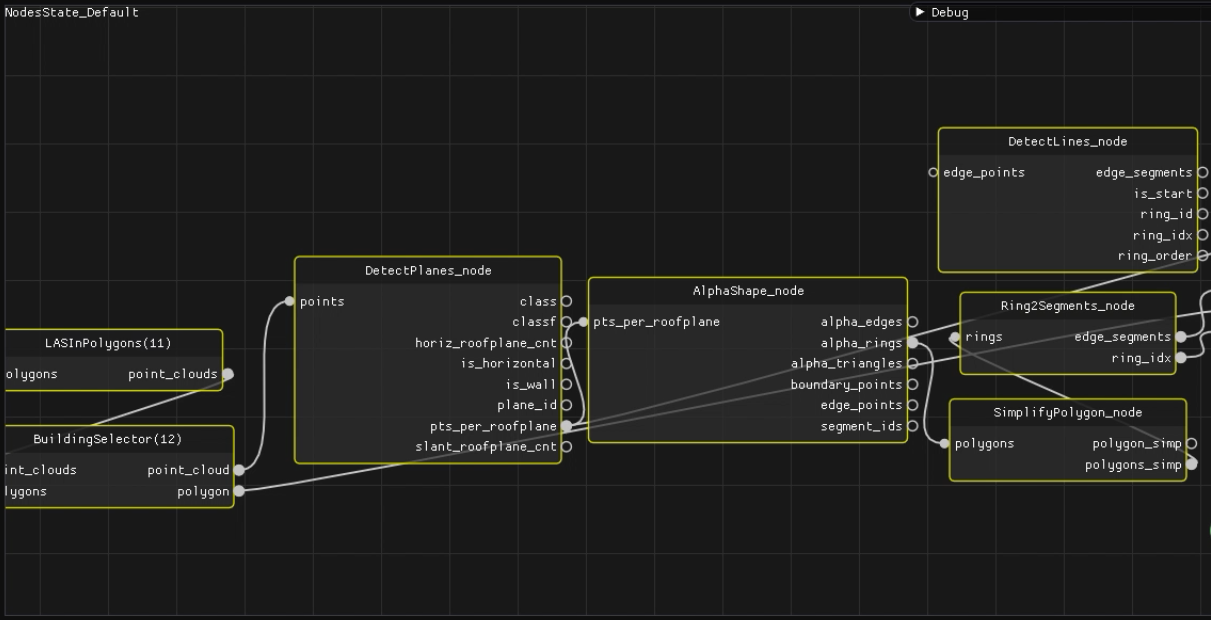
\includegraphics[width=\linewidth]{geoflow.png}
  \caption{Geoflow: A geocomputation VPL (Source)}
  \label{fig:1:geoflow}
\end{figure}

A visual programming language is a type of programming language which uses an alternative model to the textual source code of regular programming languages. 
These alternative models are represented by a \ac{GUI}, in which the program might take the shape of a graph or a block-based instruction set. 
The value a VPL lies in the fact that constructing or editing a program in a visual way can be a faster process than using a textual method, even for the most experienced software developers (Source: VPLs, Source, Vpls). 
Additionally, a \ac{VPL} allows for End User Development (Source). 
A \ac{VPL} may make processes more accessible to end users, as it allows practitioners to automate some processes and workflows like a software developer, but without needing a background in software development (Source: End user development). 

These qualities are beneficial to geocomputation, and perhaps as a consequence, geocomputation by means of visual programming is not an uncommon phenomena in the field of \ac{GIS}.
For example, Safe software's FME (SOURCE) is a popular \ac{VPL} among \ac{GIS} practitioners, arguably due to the way it simplifies the process of writing a \ac{ETL} pipeline. 
Another example is McNeel's Grasshopper (source), often used for small-scale spatial analyses, like solar irradiation or heating demands of a neighborhood (source). 

A new development regarding Geocomputation VPLs is attempting to make these VPLs web applications.
The value in this that web applications require no explicit installment to use the application (source: vpl 2019, source: hybrid). 
The Mobius Modeller is a good example of a browser-based geocomputation VPL.
The application allows users to configure a calculation by visual means in a web browser, which can then be shared as a stand-alone web application. 

%%%%%%%%%%%%%%%%%%%%%%%%%%%%%%%%%%%%%%%%%%%%%%%%%%%%%%%%%%%%%%%%%%%%%%%%%%%%%%%

% \subsection*{Shortcoming: No true dataflow programming}

% The assumption that a geo-web-vpl should be implemented as a dataflow vpl is made because of the many advantageous qualities layed out in \refsec{sec:background:dataflow}. 
% Additionally, and perhaps consequently, all comparable VPLs analyzed in \refsec{sec:related-geovpl} were implemented as dataflow VPLs (Blender, houdini, Grasshopper, GeoFlow), the only exception being the Möbius Modeller.
% However, this meant that a new, web-based implementation had to be made, since no existing web-vpl concerned with geometry uses this model (that this study is aware of).

\subsection*{Problem Statement}
  
The web based geocomputation VPL is a novel development, and contains a multitude of unaddressed challenges.
This study focusses on the particular problem of library portability. % and integration

Successful geocomputation pipelines often relies on operations found in a select number of libraries. 
Most major, industry-standard geocomputation libraries are native, C++-based libraries. 
Examples of these are GDAL, PROJ, and GEOS. 
However, A web based geocomputation VPL like the Mobius Modeller does not make use of these libraries, and has to use javascript equivalents like Turf (Source).
While it should be possible to port a library like GDAL to javascript, guarantying that these two versions show the same behavior will be complex and time consuming. This will slow down development, or create large version discrepancies. 

Fortunately, on a theoretical level, it is possible to compile a native C++ library to a web-consumable format using the 'WebAssembly' binary format.
This way, only one library needs to be maintained to serve all platforms, both native and web. 
However, no example exists of a web-based geocomputation VPLs which make use of native geocomputation libraries.

This could be because of several of reasons

It is unclear in which 

There are many aspects in between writing a native geocomputation library, and using it on the web, in a VPL format. 


This study starts from the assumption that web-based VPLs are unable to support existing geocomputation functionalities. 
This could be because of several reasons, of which this study identifies four major ones.

geocomputation functionalities might not be able to be properly:
\begin{itemize}[-]
  \item \textbf{compiled} into a format functional on the web (wasm limitations)
  \item \textbf{loaded} within a web-based VPL (bindings)
  \item \textbf{represented / visualized} by the interface of a web-based, dataflow-VPL (explain more about dataflow VPL)
  \item \textbf{used} within a web-based dataflow-VPL
\end{itemize}

As it is unknown which one of these reasons is causing this barrier, the study must cover all four of these possible hindrances, and access if and how this challenge can be overcome. 


these aspects form a hinder towards the main goal of a \ac{geo-web-vpl}. 
Moreover, the real reason might not lie in one of these areas, but in the interplay between all of these factors. 

It is this study's objective to pose a solution to this barrier. 
% This is stated by the main research question: \myMainRQ 
The study goes about doing so, by developing a prototype \ac{geo-web-vpl} accompanied by web-compiled geocomputation libraries. 
This prototype vpl is used as a staging ground to discover the extent of possible hindrances. 
% During its development, each one of these four possible hindrances has to be accounted for. 
Per hindrance, we document design considerations, and run experiments, all to test to what extent this prototype \ac{geo-web-vpl} fails or succeeds to provide for this aspect. 
After this is done, we can compile a final conclusion to the main research question. 



%%%%%%%%%%%%%%%%%%%%%%%%%%%%%%%%%%%%%%%%%%%%%%%%%%%%%%%%%%%%%%%%%%%%%%%%%%%%%%%%%%%%%%%%%%%%%%%%%%%%%%%%%%%%%%
%%%%%%%%%%%%%%%%%%%%%%%%%%%%%%%%%%%%%%%%%%%%%%%%%%%%%%%%%%%%%%%%%%%%%%%%%%%%%%%%%%%%%%%%%%%%%%%%%%%%%%%%%%%%%%
%%%%%%%%%%%%%%%%%%%%%%%%%%%%%%%%%%%%%%%%%%%%%%%%%%%%%%%%%%%%%%%%%%%%%%%%%%%%%%%%%%%%%%%%%%%%%%%%%%%%%%%%%%%%%%
%%%%%%%%%%%%%%%%%%%%%%%%%%%%%%%%%%%%%%%%%%%%%%%%%%%%%%%%%%%%%%%%%%%%%%%%%%%%%%%%%%%%%%%%%%%%%%%%%%%%%%%%%%%%%%
%%%%%%%%%%%%%%%%%%%%%%%%%%%%%%%%%%%%%%%%%%%%%%%%%%%%%%%%%%%%%%%%%%%%%%%%%%%%%%%%%%%%%%%%%%%%%%%%%%%%%%%%%%%%%%

% \begin{note}
%   TODO: make both of these presuppositions clear
%   1. Combining a geo-vpl and bbg is useful. It is valuable to figure out if it can be done properly
%   2. properly -> utilization of existing, native geocomputation libraries within a VP environment is key to making a geo-web-vpl succeed. 
% \end{note}



% Plagiarism!!!! 
% This is often addressed by maintaining multiple code bases: one web-based, usually written in JavaScript, and one for desktop and mobile, often written in C/C++. The maintenance of several code bases slows down innovation and makes evolution time-consuming. 

%%%%%%%%%%%%%%%%%%%%%%%%%%%%%%%%%%%%%%%%%%%%%%%%%%%%%%%%%%%%%%%%%%%%%%%%%%%%%%%
%%%%%%%%%%%%%%%%%%%%%%%%%%%%%%%%%%%%%%%%%%%%%%%%%%%%%%%%%%%%%%%%%%%%%%%%%%%%%%%
%%%%%%%%%%%%%%%%%%%%%%%%%%%%%%%%%%%%%%%%%%%%%%%%%%%%%%%%%%%%%%%%%%%%%%%%%%%%%%%

% Note: this are all fragments and motivations. I'm leaving them here, don't
% be bothered by them, keep things concise, but if we need extra baggage, we 
% can get it from here. 

%%%%%%%%%%%%%%%%%%%%%%%%%%%%%%%%%%%%%%%%%%%%%%%%%%%%%%%%%%%%%%%%%%%%%%%%%%%%%%%
%%%%%%%%%%%%%%%%%%%%%%%%%%%%%%%%%%%%%%%%%%%%%%%%%%%%%%%%%%%%%%%%%%%%%%%%%%%%%%%
%%%%%%%%%%%%%%%%%%%%%%%%%%%%%%%%%%%%%%%%%%%%%%%%%%%%%%%%%%%%%%%%%%%%%%%%%%%%%%%

% This design of geofront contains several challenges. Browser-based geocomputation (BBGC) might not be as performant as back-end / native geocomputation \cite{panidi_hybrid_2015, hamilton_client-side_2014}, even with the usage of WebAssembly \cite{jangda_not_2019}. 
% Additionally, since current visual programming environments all fall short on at least one of the above features, the visual programming environment will have to be created from scratch.

% The cloud-native geospatial movement represents a significant opportunity and challenge to these VPL interfaces. The \textbf{opportunity} lies in the fact that a VPL interface is highly suitable as a 'configurator' or 'IDE' for cloud-computation. The promise of interactive, low-code automation matches the desire of most cloud native geocomputation providers to support users of different backgrounds, both programmers and non-programmers, both full GIS experts as well as non-experts (SOURCE: Modellab, SOURCE: Chris Holmes). A good example of this is the ModelLab VPL, found in Raster Foundry (SOURCE). This is also evident in the fact that existing VPL's like FME and Grasshopper have added proprietary cloud-computation features like FME Cloud (SOURCE) and ShapeDiver (SOURCE), respectively.

% <!-- HOWEVERRRRRRRRR -->
% However, the major \textbf{challenge} is that as of right now and despite these developments, popular VPL's fall short on a number of priorities and features required for cloud-native geospatial computation. 
% These shortcomings include their closed and proprietary nature, their distance from regular programming features and conventions (git version control, continuous integration), and the non-containerized, one to one relationship between the IDE application \& the cloud hosting platform. All of this hinders their suitability as general, cloud-computation configurers. 


% For a geocomputation method to match the 'cloud native geospatial movement'

% Currently, WebAssembly is the only way one can take a geocomputation function from an arbitrary source, and use it in both the browser and on a server. 
% We wish to discover if this has any practical use cases. 

% - "As massive datasets become more and move available, the availability of the \emph{means} to process and analyse these data becomes more and more relevant". 

% Despite these advantages, open, accessible vpl's are often unavailable. 
% - Expensive, proprietary environments 
% - Require specific plugins in order to utilize open, industry standard geocomputation libraries
% - Not FAIR geocomputation

%%%%%%%%%%%%%%%%%%%%%%%%%%%%%%%%%%%%%%%%%%%%%%%%%%%%%%%%%%%%%%%%%%%%%%%%%%%%%%%

% This thesis explores if these in-between processing steps could also be performed within a web application.  

% This way, geodata processing applications could profit from the ease of accessibility and maintainability granted by the web as a platform.  

% <!-- More Why of web GIS and web-geocomputation: 
% - making the geoweb more feature-rich
% - allowing quick demonstration (wapm)
% - allowing easy access (overleaf)

% ## Motivation
% Under normal circumstances, Web applications within the field of geo-informatics are mostly used for the first and final stages of a common geodata process: Retrieval and visualization. 
% The processing stages in-between are almost always performed on the desktop using environments like QGIS or ArcGIS, or by writing and using CLI tools. 

% <!-- At the same time, a need arrises -->

%%%%%%%%%%%%%%%%%%%%%%%%%%%%%%%%%%%%%%%%%%%%%%%%%%%%%%%%%%%%%%%%%%%%%%%%%%%%%%%

% Under normal circumstances, Web applications within the field of geo-informatics are mostly used for the first and final stages of a common geodata process.  
% (
% If one wishes to retrieve geodata, web portals are used to discover the required datasets. After this, the OGC Web Services are often utilized to download and truly access this geodata. 

% This geodata is then processed locally, using QGIS, ArcGIS, command line tools, or any other 

% and at the end Tools like Leaflet and Celcium have been created to visualize the earth in both 2D and 3D , and tools like d3.js can produce interactive graphs to supplement these web pages. 

% There is, however, more to the web than just visualization. Due to 
% )
% This thesis asks the question if the web could do more than just visualization. 

% By creating the use-case application GeoFront, we ask the question if a modern web browser, and the current state of the client-side web technologies are capable of facilitating  

%%%%%%%%%%%%%%%%%%%%%%%%%%%%%%%%%%%%%%%%%%%%%%%%%%%%%%%%%%%%%%%%%%%%%%%%%%%%%%%

\section{Research Objective}

Two problems exist in this context: 

1. firstly, code portability. 
-> geo-web-vpl do not make use of native, industry standard geocomputation libraries

2. Secondly, existing implementations are not using a dataflow paradigm
-> functional programming, inspect parameters, 

TODO: make this more straightforward

This study seeks to close the gap between geo-VPLs and browser-based geocomputation by designing, implementing, and evaluating a new prototype \ac{geo-web-vpl}.
The study starts from the presupposition that proper utilization of existing, native geocomputation libraries within a visual programming environment is key to making a geo-web-vpl succeed. 
Overcoming this technical challenge is the focal point of this study. 

\section{Research Questions}
Based on this objective, the research question is formulated as follows: 
\begin{itemize}[ ]
  \item \myMainRQ
\end{itemize}

\subsection*{Supporting Questions}
The following supporting questions are defined to aid in answering the main question.
These are based upon various components of the main problem statements, further explained in \refchap{chap:methodology}

\begin{note}
  - first question -> you really studied it?
  - I'd remove to what extent? it's hard to answer
  - missing evaluation in questions -> performance evaluation?
\end{note}

\begin{itemize}[-]
  \item \mySubRQOne
  \item \mySubRQTwo
  \item \mySubRQThree
  \item \mySubRQFour
\end{itemize}
In order to obtain answers to these questions, a literature review is performed,
a prototypical software application is developed, 
and this application is tested and accessed on various aspects.

\newpage
\section{Scope}
The scope of this thesis is cornered in the following six ways: 

\subsection*{Only frontend geocomputation}
This study excludes any \emph {backend} based geocomputation.
A web application \textit{could} be used to orchestrate geocomputation web-services, which could also deliver a form of browser-based geocomputation to end-users. 
However, for the scope of this thesis, we limit ourselves to purely client-side solutions, with calculations literally happening within the clients browser. 
This is also why this study excludes the OGC standard of the \ac{wps} \cite{ogc_web_2015}.

Adding backend-based geocomputation to a geo-web-VPL would be an excellent follow-up investigation to this study. 
Future work could research the possibility of utilizing a hybrid strategy of both client-side and server-side geocomputation, following in the footsteps of \cite{panidi_hybrid_2015}. 

\subsection*{No Usability Comparison} % 
\begin{note}
  needs a better argument for usability -> technical feasibility only
\end{note}

While accessibility / usability is a motivation of the development of a \ac{vpl}, and while usability will be analyzed to a limited extent, no claims will be made that this method of geocomputation is \emph{more} usable as opposed to existing geocomputation methods. This research attempts to solve practical inhibitions in order to discover whether or not browser-based, vpl-based geocomputation is \emph{a} viable, usable option. If it turns out that this method is viable enough technically, future research will be needed to definitively proof \emph{how} usable it is compared to all other existing methods.  

% This paper seeks to first close this gap, limiting itself to overcoming the technical and design boundaries in the pursuit of practical client-side geocomputation.

Similarly, a survey analyzing how users experience browser-based geocomputation in comparison to native geocomputation must also be left to subsequent research. While this would be insightful, client-side geocomputation is too new to make a balanced comparison. Native environments like QGIS, FME or ArcGIS simply have a twenty year lead in research and development. 

% While the research restrains itself from empirically measuring an aspect as nebulous as 'accessibility', it does demonstrate ...


% It is my goal to introduce this as a new geocomputation option, and to name the advantages and disadvantages we can be sure of. An actual comparison of client-side vs native geocomputation is something different. 

\subsection*{Only WebAssembly-based containerization}

\begin{note}
  p.5 is backend geocomputation really browser-based geocomputation? I'd say no, could be used to shorten this section

  -> I would still include this part, when I explain my thesis to colleagues and other people, this is one of the things which comes up. Better safe than sorry.
\end{note}

This thesis examines a WebAssembly-based approach to containerization and distribution of geocomputation functionalities. 
Containerization using Docker is also possible for server-side applications, but is not (easily) usable within a browser. 
For this reason, Docker-based containerization is left out of this studies' examination. 
And to clarify: Docker and WebAssembly are not mutually exclusive models, and could be used in conjunction on servers or native environments. 

\subsection*{Mostly Point Cloud/ DTM focussed geocomputation}
We are also required to concentrate the scope of 'geocomputation', which is a sizable phenomenon.
The term is generally used to cover all operations on geodata, from rasters, tabular datasets, highly structured datasets such as the CityJSON or IndoorGML, and point clouds. 
Due to time limitations, we are forced to focus on particular type of geocomputation.
3D-based geocomputation is chosen, with a particular focus on pointclouds and DTMs. 
The hypothesis is that these types of data may fit the small-scale geocomputation of a 'geo-web-vpl' well due to the local optimality quality of many DTM procedures (Such as the \ac{dt}), 

\subsection*{Assumption: a '\ac{geo-web-vpl}' is a normal Geometry VPL able to handle geodata}
For the scope of this thesis, we assume a Web-VPL for geocomputation is practically the same as a web-VPL for generic geometry processing.
Examples of "Geometry VPLs" are Blender's Geometry Nodes, Houdini, GeoFlow, and Grasshopper.
More on this in chapter \refsec{sec:related-geovpl}.

A geo-web-vpl differs only in the fact that it supports additional geodata types, and offers functionalities specific to processing those types.  
This assumption is safe to make since a 'geo-web-vpl' will \emph{at the very least} require the same features as a 'normal' geometry VPL, due to their common dependency on the field of computer graphics and computational geometry.

Still, in reality, a lot of differences and nuances exist between the field of geocomputation and the field of procedural modelling. 
However, due to time limitations, these concerns are left to future research.
% these concerns will only be picked up at the final discussion, found at \refsec{sec:discussion}.
 
\subsection*{Only core browser features}
Lastly, the implementation of the geo-web-vpl will limit itself to core browser features, keeping dependencies at a minimum, in an attempt to generalize the results of the study.
If the study would use very specific web frameworks and technologies to solve key issues, questions might arise if the results of the study counts in general for browser-based geocomputation or geo-VPLs, or if they only count in this very specific scenario. 
"Core browser features" is defined in \refsec{sec:method-one}.

\newpage
\section{Reading Guide}
The remainder of this study is structured as follows:

\begin{itemize}[ ]
  \item \refchap{chap:background}, Background, provides an overview of the theoretical background that is used in the rest of this study.
  
  \item \refchap{chap:related}, Related Work, provides a review of studies comparable to this one.

  \item \refchap{chap:methodology}, Methodology, explains precisely in what way the research-questions will be answered, and shows how this relates to the background and related works chapters. 

  \item \refchap{chap:implementation}, Implementation, presents the implementation of the methodology.
  In addition, the main design decisions are described and justified in this part of the study.
  
  \item \refchap{chap:analyses} analyses the results from this implementation in the various ways described by the methodology.
  
  \item And finally, \refchap{chap:conclusion}: Conclusion \& Discussion, concludes to which extent the study was able to satisfy the main research question, and discusses unaddressed aspects of the thesis.
  It also includes the envisioned future works and a reflection on the quality of the study.

\end{itemize}